\href{http://www.weltenbau-wissen.de/2016/02/5-rezepte-fantasy-kulturen-zivilisationen/}{Fantasy-Zivilisationen}

\chapter{Religion}
\section{Übersicht}
\begin{itemize}
	\item Der Glaube an 5 gute und 2 böse Götter.
	\item Das Symbol der Religion ergibt sich wie in Abschnitt \ref{sec:goettersymbol} erklärt aus dem Zusammenspiel der 7 Götter und ist in Bild \ref{fig:goettersymbol} dargestellt.
\end{itemize}

\begin{figure}
	\centering
	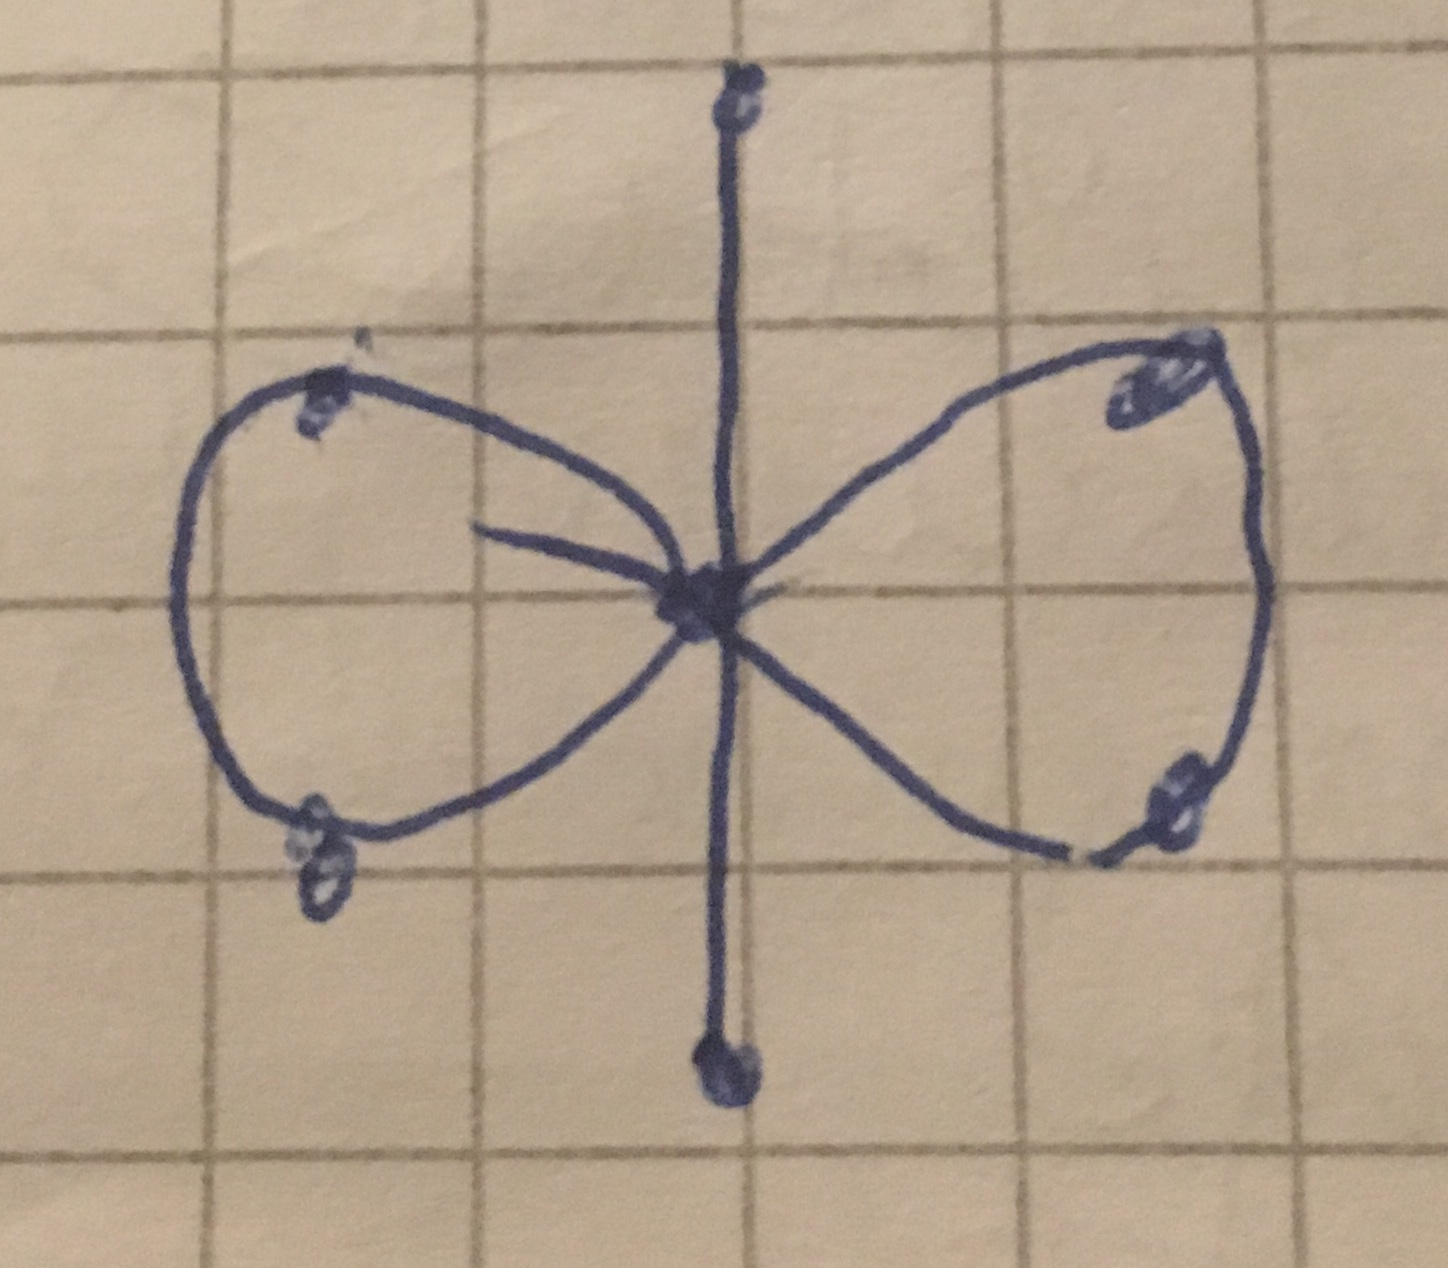
\includegraphics[width=0.3\textheight]{Abbildungen/Gesellschaft/Goettersymbol}
	\caption[Göttersymbol]{Das Symbol für die Götter}
	\label{fig:goettersymbol}
\end{figure}

\section{Geschichte}
Die hier erzählte Geschichte ist die vom Klerus verbreitete Sage über die Entstehung der Götter des Streits und der Heimtücke. \\\\
Es ist unklar, wie die Götter entstanden sind. Es geschah irgendwie irgendwann. Auf der noch recht unbewohnbaren Erde formten sie lebensfreundliches Gebiet mit ihrer jeweiligen Magie. Sie erschufen das Leben und ließen ihm seinen eigenen Lauf.\\
Nachdem sie jedoch viel Zeit damit verbracht hatten, sich an ihrem Paradies zu ergötzen, wollten sie auch Wesen nach ihrem Abbild schaffen und so lenkten sie das Leben und die Natur und brachten dadurch die Menschen hervor. Die Menschen, intelligent genug um Kultur aufzubringen, verfielen jedoch in viele Kriege. Mitgerissen aufgrund ihrer Ähnlichkeit und weil sie die Menschen so interessant fanden, integrierten sich die Götter in diese Streitigkeiten. Dabei nahmen sie die Positionen ihrer Menschengruppen an und halfen ihnen und wurden so langsam auch in einen Streit untereinander gezogen, wobei sie ihre negativen Seiten ausspielten.\\
Dies äußerte sich in vielen kleinen Dingen \textbf{(hier Geschichtchen einfügen)}, bis die Götter schließlich merkten, dass es so nicht weiter gehen kann. Sie setzten sich zusammen und kamen zum Schluss, dass sie, um wahre Leiter und Lenker des Lebens zu sein, ihre negativen Aspekte los werden müssten. Andernfalls würden ihre dunklen Seiten sie immer wieder übermannen können, was bereits große negative Folgen für alle Lebewesen hatte und auch wieder haben könnte.\\
Darum bereiteten die Götter ein Ritual vor, um perfekt zu werden und sich wortwörtlich von ihren schwachen Seiten rein zu waschen. Dazu begaben sie sich in einen See weitab der Zivilisation. Sie wuschen ihre schlechten Seiten von sich ab und versiegelten diese im See. \textbf{Allerdings gibt es ein kleines Leck, durch welches kontinuierlich ein wenig von der Magie und dem Schlechten austritt.}\\
Danach treten die Götter lange Zeit nicht in Erscheinung. In der Nähe des Sees, den Bach hinunter, lebte ein Paar. All sein Trinkwasser nahm es aus dem Bach und all ihre Ernte wurde mit dem Wasser bewässert. So nahmen sie über Zeit immer mehr von dem Bösen in sich auf. So wie ihre Macht und Magie wuchs, tat es auch das Böse in ihnen und verzehrte ihre guten Geister. Sie begannen aktiv das Böse aus der Umwelt und schließlich dem See zu absorbieren und wurden immer mächtiger und verdorbener. Sie führten Verwüstung und Zwist herbei und die Götter wurden auf sie aufmerksam. Ihre Versuche, sie zu bekämpfen und unter Kontrolle zu bekommen, scheiterten unter großen Verlusten in der Umwelt. Schließlich sahen die Götter ein, dass sie die beiden nicht besiegen konnten und unter all ihrer gebündelten Macht, um alle Lebewesen zu schütze, ersannen sie einen radikalen Plan.\\
Da die Götter zu verantworten hatten, dass diese Monster auf die Welt kamen, sahen sie es als ihre Pflicht, die Welt auch wieder von ihnen zu befreien. Aufgrund der zuvor genannten Umstände war die Maßnahme jedoch von drastischer Natur: sie hoben den Ort, auf dem sie die beiden bekämpften, aus der Erde heraus in den Himmel. Dort werden sie nun für alle Zeit gegen die beiden kämpfen und sie in Schach halten, damit das Leben auf der Erde geschützt ist.\\
Doch die beiden Bösen versuchen ihre Macht zu vergrößern, indem sie ihre Aktuelle auch dazu nutzen, den Lebewesen auf der Erde Böses einzuflüstern und sie zu manipulieren. \textbf{Die Erdenwesen sollen ihnen dienen.}\\
Bevor die guten Götter die Erdmasse mitsamt den Bösen in den Himmel aufgehoben haben, \textbf{erschufen sie gemeinsam einen Führer für die Toten}, der die verstorbenen Seelen zu ihnen bringen soll. Im Laufe der Zeit, in der sie ihre Pflichten als Götter und Führer der Welt etwas außen vor ließen, haben sie es geschafft, die Bösen zurück zu treiben. Nun gibt es nur noch Kampf auf einem kleinen Teil des Himmels-Brockens.\\
Nachdem die Toten verbrannt wurden, steigen ihre Seelen in den Himmel auf. Wenn die Verstorbenen in ihrem Leben gut waren und sich nicht von den Einflüsterungen der bösen Götter haben verführen lassen, werden sie vom Seelenleiter hinüber geführt, auf dass sie mit ihrer Kraft die Götter unterstützen und in ihrem Paradies wohnen können. Die verdorbenen Seelen jedoch werden vom Seelenleiter in die Irre geführt, damit sie nicht den Bösen helfen können, und verlieren sich in der unendlichen Dunkelheit.

\section{Götter}
In dem Land, in dem wir uns befinden, gibt es mehrere Götter. Regional unterscheidet sich die Wahl der bevorzugten Götter.
Diese sind Fiktion und existieren nicht wirklich; es gibt also auch keine Wunder, die von ihnen gewirkt werden. Allerdings interpretieren Menschen ja gerne sehr viel und sehen deshalb ein paar Dinge als Wunder an, die z.B. von den Priestern gemacht werden. Weil diese Priester gute Magier sind, aber das alles natürlich als Geschenk der Götter sehen.\\

Die Ausführungen im Folgenden stellen den Pantheon dar, wie er zur Zeit des Spiels angebetet wird. Alle Namen sind vorläufig und mehr Möglichkeit gesehen, den Göttern und 
benannten Orten etwas mehr Griffigkeit zu geben. Die Details, die im Folgenden gegeben werden (insbesondere die beispielhafte Mythen und Erzählungen über die Götter) dienen 
der Anschaulichkeit für uns und müssen sich nicht zwingend im Spiel wiederfinden.

\subsection{\textbf{Asdar} - Gott der Führung und des Schutzes}
Asdar ist der Anführer der Götter - nicht aufgrund außergewöhnlicher Stärke oder Charisma - Asdar ist nicht mächtiger als seine Mitgötter, sondern weil es seinem Wesen entspricht. Asdar ist standhaft, mutig und 
vertritt Führung durch Vorbild. Da, wo die Schutzbedürftigen verteidigt oder Verlorenen angeleitet werden müssen, ist Asdar in der ersten Reihe zu finden. \\
\begin{itemize}
	\item Aussehen 
	\begin{itemize}
		\item großer Mann im mittleren Alter
		\item kurze silberne Haare
		\item häufig in Rüstung und mit alten Kampfnarben
	\end{itemize}
	\item Aspekte
	\begin{itemize}
		\item Herrschaft und Führung
		\item Kampf und Schutz
		\item Vertreibung von Übel
	\end{itemize}
	\item Tugenden Asdars
	\begin{itemize}
		\item Standhaftigkeit, Mut
		\item körperliche Stärke und Macht
		\item Opferbereitschaft
	\end{itemize}
\end{itemize}
\textit{Weit bekannter Mythos Asdars}:\\
Vor Urzeiten, als die Welt noch jünger war, streiften mächtige Monster durch die Lande und verbreiteten Angst und Schrecken. Es begab sich, dass Asdar, als einfacher Wanderer 
verkleidet, in einem Dorf Herberge suchte. Ein Lindwurm, eine mächtige Bestie mit einer geschuppten Haut härter als Stein und Klauen und Zähnen größer und schärfer als das 
beste Schwert der Menschen, fiel über das Dorf her, getrieben von unstillbarer Gier und Hunger. Und Asdar offenbarte sich in seiner Rüstung und sprach: ``Wer bereit ist, sein Heim 
und seine Familie zu verteidigen, der nehme seine Waffe und kämpfe an meiner Seite.'' Und die Menschen folgten seinem Ruf, gewappnet mit jedweder Waffe die sie finden konnten. 
Der Kampf war lang und schwierig und manch einer wäre dem Hunger des Wurms zum Opfer gefallen, wenn Asdar die Angriffe nicht mit Schild und Rüstung abgefangen hätte. Und 
mit seinem letzten Atemhauch gelang es dem Lindwurm noch, Klaue an Asdar zu legen und ihm eine weitere Narbe zu verpassen.

\subsection{\textbf{Bouda} - Göttin der Harmonie und des Wachstums}
Bouda ist die schaffende Gottheit des Pantheons. Nach ihrem Willen erwachsen neue Pflanzen in jedem Frühling, um den Hunger aller zu stillen. Nach ihrem Wilen wir das Band 
der Ehe geformt, das Mann und Frau in Harmonie miteinander verbindet. Bouda akzeptiert alle als ihre Kinder und schenkt die Fähigkeit, zu vergeben und zu versöhnen.\\
\begin{itemize}
	\item Aussehen 
	\begin{itemize}
		\item ``Mutterfigur''
		\item mittleres Alter 
		\item kräftige Figur
		\item alltägliche Kleidung 
	\end{itemize}
	\item Aspekte
	\begin{itemize}
		\item Familie (Ehe und Elternschaft)
		\item Ernte und Wachstum
		\item Heilung
	\end{itemize}
	\item Tugenden Boudas
	\begin{itemize}
		\item Gnade und Demut
		\item Offenheit und Akzeptanz
		\item nichterotische Liebe
	\end{itemize}
\end{itemize}
\textit{Weit bekannter Mythos Boudas}:\\
Vor Urzeiten, als die Welt noch jünger war, lagen die Reiche der Menschen beständig im Streit miteinander. Päkte wurden geschmiedet und gebrochen, ein Herrscher folgte auf den 
nächsten und keiner vermochte es, andauernden Frieden zu finden. Doch manchmal schmiedete das Schicksal seltsame Bande: es begab sich nämlich, dass die Thronfolger zweier 
verfeindeter Reiche in demselben Wald jagten und von einem Sturm von ihren jeweiligen Wegen abgebracht und in der 
Hütte einer alten Frau zusammengebracht wurden. Und als die beiden sich der Anziehung bewusst wurden, die zwischen ihnen zu erblühen begann, baten sie die alte Frau, ihre
Vermählung vor Bouda zu bezeugen, auf dass selbst ihre Väter sie nicht mehr trennen könnten. Und die alte Frau schenkte ihnen zur Mitgift zwei Armreife, die das Band ihrer Vereinigung 
darstellen sollten. Und als die beiden Thronfolger heimkehrten, kam Friedfertigkeit über jeden, der die Reife der beiden sah. Und zum ersten Mal seit langem herrschte Frieden 
zwischen den Nationen.

\subsection{\textbf{Erlin} - Gott des Ausgleichs und der Gerechtigkeit}
Erlin lehrt die Menschen, die Bindungen zu ihren Mitmenschen ausgewogen zu halten. Sowohl Respektlosigkeit als auch übermäßige Ehrerbietung versäuern das Verhältnis 
zu den Mitmenschen und muss daher vermieden werden. Dazu gehört sich an die Gesetze und Regln der Gesellschaft zu halten.\\
\begin{itemize}
	\item Aussehen 
	\begin{itemize}
		\item alter Mann 
		\item hochgewachsen und hager
		\item in makelloser Robe, aufrechte Haltung
		\item Richthammer am Gürtel
	\end{itemize}
	\item Aspekte
	\begin{itemize}
		\item Gesetzgebung und Rechtsprechung
		\item Handel
		\item Weises Vorgehen \footnote{Leichte Überschneidung mit Faelans Aspekt}
	\end{itemize}
	\item Tugenden Erlins
	\begin{itemize}
		\item Disziplin und Respekt
		\item stoisch und gelassen
		\item streng mit sich selbst und Anderen
	\end{itemize}
\end{itemize}
\textit{Weit bekannter Mythos Erlins}:\\
<Erlin fällt eine Richtspruch über ...>

\subsection{\textbf{Aina} - Göttin der Lebensfreude und Liebe}
Aina mag für manche wie die schwächste der Götter aussehen - ihre Mythen berichten fast ausschließlich von Festen und Kunstwerken. Und dennoch ist Aina eine der beliebtesten 
Götter im einfachen Volk. Jeder Reigen zum Mittsommerfest, jedes alkoholschwangere Fest und jeder stille (und jeder weniger stille) Moment der Zweisamkeit genießt Ainas Segen 
und Unterstützung.\\
\begin{itemize}
	\item Aussehen 
	\begin{itemize}
		\item junge Frau in Festtagskleidung
		\item häufig zum Lachen aufgelegt
		\item attraktiv 
	\end{itemize}
	\item Aspekte
	\begin{itemize}
		\item erotische Liebe (als Vereinigung)
		\item Feierlichkeiten
		\item Kunst und Kultur
	\end{itemize}
	\item Tugenden Ainas
	\begin{itemize}
		\item Kreativität und Freigeistigkeit
		\item zu Scherzen aufgelegt
		\item charmant und fröhlich
	\end{itemize}
\end{itemize}
\textit{Weit bekannter Mythos Ainas}:\\
Vor Urzeiten, als die Welt noch jünger war, waren die Menschen eitel aufgrund ihrer eigenen Fertigkeiten. Glemric, Barde und Meister seiner Zunft, war einer dieser Menschen. 
Er rühmte sich seiner Künste mit Flöte und Harfe und behauptete, dass selbst Aina selbst nicht mit ihm mithalten könne. Und so kam es, dass eines Abends, als die Nächte 
kurz und der Mittsommer nahe war, eine junge Frau vor seiner Tür stand und ihn zu einem Wettbewerb herausforderte. Gäste wurden geladen, um die Kunstfertigkeit der Kontrahenten 
zu bewerten und sich ihrer Kunst zu erfreuen. Doch jedes Stück, das Glemric aufspielte, vermochte sein Gast zu überbieten, bis letzlich sogar Glemric selbst einsehen musste, 
dass er geschlagen war. Noch an diesem Abend gelobte er, seine Ehre wiederherzustellen und sich bei seinem Gast zu revanchieren. Und so geschah es, dass Glemric ein Jahr später 
in derselben Nacht Aina zu einer Revanche herausforderte. 

\subsection{\textbf{Faelan} - Gott der Schläue und des Glücks}
Weisheit kann viele Dinge bedeuten. Die Fähigkeit, Zusammenhänge zu begreifen und auszunutzen. Die Fähigkeit, den für sich selbst und Andere besten Weg zu erkennen. Und die 
Fähigkeit, aus dem Wenigen, was man hat, das Beste zu machen. Faelan verkörpert diese Fähigkeiten auf seine Art und Weise. Er hat weder Asdars Stärke noch Erlins Urteilsvermögen - 
und dennoch ist er regelmäßig in der Lage, die beiden auszutricksen und ihnen dennoch keinen bleibenden Schaden zuzufügen.\\
\begin{itemize}
	\item Aussehen 
	\begin{itemize}
		\item Junger Mann 
		\item schlank und gelenkig
		\item beständig grinsend
	\end{itemize}
	\item Aspekte
	\begin{itemize}
		\item Weisheit als Schläue und List
		\item Glück und Überwindung von Herausforderungen
		\item Reisen 
	\end{itemize}
	\item Tugenden Faelans
	\begin{itemize}
		\item Scherze 
		\item Bewusstsein der Unzulänglichkeit
		\item überlegtes und zielstrebiges Vorgehen
	\end{itemize}
\end{itemize}
\textit{Weit bekannter Mythos Faelans}:\\
<Faelan stiehlt Erlin Richthammer>  


\subsection{\textbf{Der Wispernde Schatten} - Gott der Heimtücke}
männlich\\
positive Aspekte: \\
negative Aspekte: 
\subsection{\textbf{Drayl} - Göttin des Streits}
weiblich\\
positive Aspekte: \\
negative Aspekte: 

\subsection{Das Göttersymbol} \label{sec:goettersymbol}
Beim Wasser-/Reinigungsritual, dem Abtrennungsritual oder einem anderen war die Aufstellung der fünf Götter und ihr Energiefluss wie dargestellt in Abb. \ref{fig:goetteraufstellung}. Denn die stärksten und direktesten Verbindundungen/Folgen ihrer Aspekte sind so. Das ergibt eine liegende acht, also das Symbol für Unendlichkeit --> 8 als heilige Zahl; Götter und ihre Macht sind unendlich.\\
\\
Mit den zwei Bösen Göttern: diese versuchen, alles zu spalten und zu zerstören. Das wird deutlich durch die Linie, welche die 8 versucht zu zerschneiden. Zudem zeigt es aber auch, wie durch die bösen Götter und zum Schutz des Lebens, ein Stück von der Erde abgetrennt werden musste. Des Weiteren mahnt es, wie unsere Schlechten Seiten immer Versuchung und Untergang sind — aber sie sind auch ein Teil von uns und wir müssen lernen, damit umzugehen und ihnen zu widerstehen. Aus diesen Aspekten ergibt sich das endgültige Göttersymbol wie dargestellt in Abb. \ref{fig:goettersymbol}.\\

\begin{figure}
	\centering
	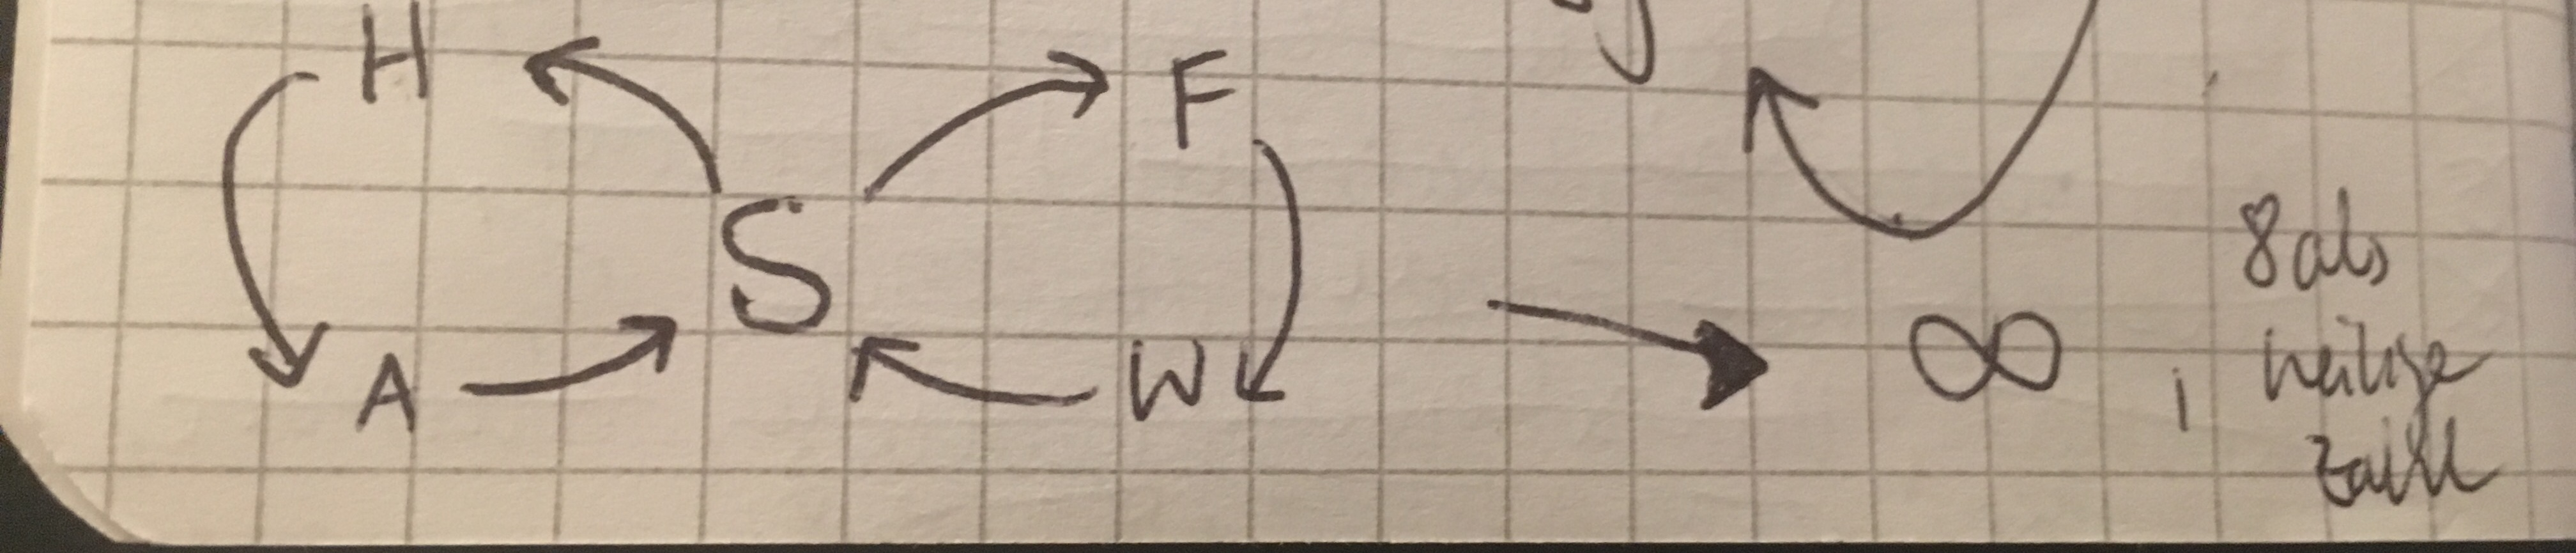
\includegraphics[width=0.7\linewidth]{Abbildungen/Gesellschaft/GoetteraufstellungbeiReinigungsritual}
	\caption{Aufstellung der Götter während des Reinigungsrituals}
	\label{fig:goetteraufstellung}
\end{figure}

\section{Klerus}
\textbf{Hier soll eine genauere Beschreibung des tatsächlichen Klerus erfolgen, also dem Teil der Struktur, der die Inhalte der Religion übermittelt. Zum Teil, der das Land verwaltet, siehe bitte \npref{ch:regierung}.} 

Da die Fähigkeit zur Nutzung der Magie natürlich auch von den Göttern kommt (nur wenige Arten können dies, ein paar Pflanzen, ein paar Tiere und darunter die menschlichen Arten (und unbekannterweise natürlich auch Mikroorganismen)), ist die Intensität, in der man Magie nutzen kann, natürlich auch ein Zeichen für die Gunst der Götter. Demnach müssen solche Leute stark in der Gunst stehen und daher auch ihr Leben den Göttern widmen - aka in den Orden gehen. Tatsächlich ist das aber auch ein Mittel des Ordens, diese mächtigen Leute zu kontrollieren, da sie die nach ihrer Art prägen und unter ihrer Anweisung haben

\subsection{Aufbau \& Struktur}

\subsection{Riten}
\paragraph{Ideen}
\begin{itemize}
	\item Predigt --> worshipping mit Gesang
\end{itemize}

\subsubsection{Tod}
Wenn jemand stirbt, so muss er verbrannt werden, damit seine Seele vom Körper frei wird und in den Himmel zu den Göttern aufsteigen kann und ihnen im Kampf gegen die bösen Götter beistehen kann. Das sollte optimal dann erfolgen, wenn die zweite Erde am Himmel steht, damit er schnell dort hingelangt. 
Gotteslästerer und böse Leute werden nicht verbrannt, sondern begraben oder ins Wasser geworfen (offenes Meer). So können sie den Bösen Göttern nicht beistehen.
Demnach ist es sehr schlimm, wenn jemand nach seinem Tod nicht angemessen aufbereitet und vor allem verbrannt wird!

\subsection{Gebäude}
